\documentclass[journal]{IEEEtran}
\usepackage{lmodern}

\usepackage{amsmath,amssymb,amsfonts}
\usepackage{textcomp}
\usepackage{xcolor}
\usepackage{booktabs}
\usepackage{multirow}
\usepackage{url}
\usepackage{hyperref}
\usepackage{balance}
\usepackage{graphicx}
\usepackage{listings}
\lstset{basicstyle=\small\ttfamily,breaklines=true,frame=single,backgroundcolor=\color{gray!10}}

\begin{document}

\title{Semantic Label Hallucination in Fine-Tuned Large Language Models: A Dual-Metric Evaluation Framework for SOC Alert Classification}

\author{
\IEEEauthorblockN{Nutthakorn Chalaemwongwan}
\IEEEauthorblockA{Department of Computer Engineering, KOSEN-KMITL\\
King Mongkut's Institute of Technology Ladkrabang\\
Bangkok, Thailand\\
nutthakorn.ch@kmitl.ac.th}
}

\maketitle

\begin{abstract}
Fine-tuning large language models (LLMs) for Security Operations Center (SOC) alert classification has become a promising approach for automating threat analysis. We present a thorough benchmark of 7 fine-tuned LLMs (0.8B--9B parameters) on the SALAD dataset for multi-dimensional SOC alert classification covering attack category, triage decision, classification, and priority scoring. Our key finding challenges the prevailing narrative of universal LLM superiority: while most models achieve perfect \emph{semantic} accuracy (normalized F1 = 100\%), \textbf{strict label compliance varies from 74.9\% to 100\%} depending on model architecture. Models with stronger reasoning capabilities (DeepSeek-R1, Phi4-mini) follow label schemas exactly, while others hallucinate MITRE ATT\&CK sub-category names from pre-training knowledge---predicting ``Port Scanning'' instead of ``Reconnaissance'' in up to 4,947 out of 9,851 test samples. We introduce the \emph{strict vs.\ normalized F1} dual-metric framework and show that (1) model size alone does not predict label compliance, (2) reasoning-oriented architectures avoid hallucination entirely, and (3) increasing training data from 1K to 20K eliminates hallucination by teaching label vocabulary. Training cost is only \$3.72 per model, making fine-tuning 149--181$\times$ cheaper than commercial LLM APIs while achieving superior accuracy.
\end{abstract}

\begin{IEEEkeywords}
SOC alert classification, LLM fine-tuning, label hallucination, MITRE ATT\&CK, strict evaluation, QLoRA
\end{IEEEkeywords}

%% ===== INTRODUCTION =====
\section{Introduction}

Security Operations Centers (SOCs) serve as the primary defense layer in organizational cybersecurity, responsible for monitoring network traffic, triaging alerts, and coordinating incident response. The scale of this task is staggering: industry surveys report that enterprise SOCs process between 10,000 and 150,000 alerts daily, with false positive rates ranging from 25\% to 50\%~\cite{ponemon2023}. This volume overwhelms human analysts, contributing to burnout and alert fatigue that allows critical incidents to go undetected for hours.

The classification of security alerts is a multi-dimensional problem that goes beyond simple binary detection. Following the NIST Cybersecurity Framework, SOC analysts must simultaneously determine: (1) whether traffic is malicious (\emph{classification}), (2) what response action to take (\emph{triage}), (3) which attack technique is being employed (\emph{attack category}), and (4) how urgent the threat is (\emph{priority scoring}). Traditional approaches handle these dimensions independently with separate classifiers, but LLMs offer the compelling possibility of unified, multi-dimensional classification in a single inference pass.

Large language models (LLMs) have emerged as a promising solution for automating SOC alert classification. Recent studies report impressive F1 scores above 95\% on cybersecurity classification tasks~\cite{ferrag2024,motlagh2024}, suggesting that LLMs can effectively replace or augment human analysts. However, these results typically rely on \emph{normalized} evaluation metrics that map semantically equivalent but lexically different predictions to the same label.

When we apply \emph{strict} evaluation---requiring exact label matches against the ground-truth schema---the picture changes dramatically. We discover a phenomenon we term the \textbf{label gap}: fine-tuned LLMs understand SOC alert categories perfectly but often express this understanding using the wrong vocabulary. A model fine-tuned on SALAD data with the label ``Reconnaissance'' will predict ``Port Scanning''---the MITRE ATT\&CK sub-technique name---because this more specific term exists in its pre-training corpus. This is not a classification error; it is a \emph{label compliance failure} driven by pre-training knowledge overriding fine-tuning.

This distinction has critical implications for production deployment:
\begin{itemize}
\item Downstream automation pipelines (SOAR, ticketing, escalation) expect exact label strings.
\item Hallucinated labels create unmapped categories that break rule-based integrations.
\item A model that ``understands'' but ``mislabels'' requires different mitigation than one that is genuinely confused.
\item SOC dashboards that aggregate alerts by category will show phantom threat categories, distorting the organization's threat landscape visibility.
\end{itemize}

To our knowledge, no prior study has examined the gap between semantic accuracy and label compliance in fine-tuned LLMs for classification tasks. This gap is invisible under standard evaluation practices but critical for deployment.

This paper makes five contributions:
\begin{enumerate}
\item \textbf{Multi-model benchmark}: We evaluate 7 models (0.8B--9B) across 4 classification dimensions on clean, zero-overlap data splits, with strict and normalized F1 reported for all.
\item \textbf{Dual-metric framework}: We introduce the strict vs.\ normalized F1 evaluation with formal definitions (\S\ref{alg:eval}) that separates semantic understanding from label compliance, revealing hidden failures in state-of-the-art models.
\item \textbf{Hallucination taxonomy}: We categorize 10,093 label errors across all models into 6 types (sub-technique, plural, cross-category, corrupted token, sibling class, augmented form) and identify architectural factors that prevent them.
\item \textbf{Non-monotonic scaling}: We demonstrate that hallucination follows a surprising non-monotonic curve with training size (5K is worse than 1K), providing the first evidence of a ``knowledge activation valley'' in fine-tuning.
\item \textbf{Cost analysis}: We show fine-tuning costs \$0.60--\$3.72 per model, making it 149--181$\times$ cheaper than commercial LLM APIs (GPT-4o: \$556, Claude Opus: \$672 per test set).
\end{enumerate}

The remainder of this paper is organized as follows: Section~II reviews related work across LLMs for cybersecurity, hallucination research, and evaluation methodology. Section~III describes our methodology, including the SALAD dataset, model configurations, and the dual-metric framework with formal definitions. Section~IV presents results across the 7-model benchmark, hallucination taxonomy, scaling analysis, and statistical tests. Section~V discusses implications for production deployment, generalizability, and threats to validity. Section~VI concludes with key takeaways and future directions.

%% ===== RELATED WORK =====
\section{Related Work}

\subsection{LLMs for Cybersecurity}
The application of LLMs to cybersecurity has grown rapidly, building on the transformer architecture~\cite{vaswani2017} and pre-trained language models such as BERT~\cite{devlin2019} and GPT~\cite{radford2019}. SecureBERT~\cite{aghaei2023} demonstrated domain-specific pre-training on vulnerability descriptions, achieving state-of-the-art NER on cybersecurity text. CyberGPT~\cite{alshaer2024} applied GPT-4 for threat intelligence extraction from unstructured reports. Ferrag et~al.~\cite{ferrag2024} provided the most thorough survey, covering LLMs across 6 cybersecurity task categories and finding that domain adaptation significantly outperforms zero-shot prompting. Motlagh et~al.~\cite{motlagh2024} benchmarked ChatGPT on 5 datasets, reporting variable performance (45--92\% F1) depending on task complexity. Zhao et~al.~\cite{zhao2023} provide a broader survey of LLM capabilities and limitations, noting that evaluation methodology remains a significant challenge across domains.

More recent work has focused on parameter-efficient approaches. CyberLLM-FINDS~\cite{cyberllm2025} combined instruction-tuned fine-tuning with retrieval-augmented generation (RAG) for MITRE ATT\&CK evaluation. Abualkishik et~al.~\cite{abualkishik2025} showed that QLoRA-based modular NIDS achieved 86\% training time reduction. Huang and An~\cite{huang2025} proposed a modular NIDS architecture leveraging QLoRA with textual representation. Lavi and Manor~\cite{lavi2024} fine-tuned LLMs for network traffic analysis, significantly outperforming non-fine-tuned baselines. However, none distinguished between semantic accuracy and label compliance---the central contribution of our work.

\subsection{SOC Alert Classification}
Traditional SOC automation relies on rule-based SIEM systems (Splunk, QRadar, ArcSight) that match alerts against predefined patterns~\cite{ponemon2023}. Machine learning approaches have shown promise: Al-Rakhami et~al.~\cite{alrakhami2022} achieved 93\% accuracy with ensemble methods on UNSW-NB15. Moustafa and Slay~\cite{moustafa2016} created the UNSW-NB15 dataset that forms the foundation of SALAD. Li et~al.~\cite{li2024} applied transformer-based models to network intrusion detection, achieving 97\% accuracy. Kim et~al.~\cite{kim2024} fine-tuned LLMs for network traffic analysis, significantly outperforming non-fine-tuned models. Arp et~al.~\cite{arp2022} highlighted critical pitfalls in ML-based security, including temporal bias and label leakage---concerns we address through our zero-overlap data splits. Apruzzese et~al.~\cite{apruzzese2023} provided an extensive survey of deep learning for network intrusion detection, noting that evaluation methodology varies widely across studies.

A critical gap in all these studies is the evaluation methodology: none report strict vs.\ normalized metrics, making it impossible to determine whether high F1 scores reflect genuine label compliance or merely semantic understanding with alias mapping.

Recent deep learning approaches have leveraged foundation models~\cite{brown2020,touvron2023} adapted through fine-tuning, shifting the paradigm from task-specific architectures to general-purpose models. Wei et~al.~\cite{wei2022} showed that chain-of-thought prompting enables reasoning in LLMs, which may explain why reasoning-oriented models avoid label hallucination in our experiments. Ouyang et~al.~\cite{ouyang2022} demonstrated that RLHF alignment training teaches models to follow instructions precisely---a capability directly relevant to label compliance.

\subsection{LLM Hallucination}
Hallucination in LLMs has been extensively studied for factual generation~\cite{ji2023,huang2023}, question answering~\cite{maynez2020}, and summarization~\cite{cao2022}. Recent advances include NoiseFiT~\cite{noisefit2025}, which uses adaptive noise injection during fine-tuning to reduce hallucination rates. Gekhman et~al.~\cite{gekhman2024} made a particularly relevant finding: fine-tuning on new knowledge can paradoxically \emph{increase} hallucination tendency, consistent with our observation that 5K training produces more errors than 1K. The SemEval-2025 Mu-SHROOM shared task~\cite{mushroom2025} addresses hallucination span detection in multilingual settings, receiving 2,618 submissions from 43 teams.

However, hallucination in \emph{classification tasks}---where models produce semantically correct but schema-violating labels---has received virtually no attention. Xu et~al.~\cite{xu2024} showed that hallucination patterns differ significantly between generation and classification settings, and Chowdhury et~al.~\cite{chowdhury2024} demonstrated that fine-tuning can both mitigate and exacerbate hallucination depending on the training distribution. We identify this novel form as \emph{label vocabulary hallucination} and provide the first systematic taxonomy.

\subsection{Parameter-Efficient Fine-Tuning}
The key insight behind LoRA~\cite{hu2022} is representing weight updates as a low-rank product $\Delta W = BA$ (with $B, A$ of rank $r \ll d$), which reduces the number of trainable parameters from $d^2$ to roughly $2dr$ per adapted layer. QLoRA~\cite{dettmers2023} extends this by applying 4-bit NormalFloat quantization to the frozen base weights, making it feasible to fine-tune models with 7B+ parameters on hardware that would otherwise be insufficient. Hsu et~al.~\cite{safelora2024} introduced Safe LoRA at NeurIPS 2024, projecting LoRA weights into a safety-aligned subspace to mitigate safety degradation during fine-tuning. While prior work focuses on accuracy-efficiency tradeoffs, we demonstrate that LoRA hyperparameters (rank, learning rate) directly impact label compliance behavior, independent of semantic accuracy.

\subsection{Evaluation Methodology}
Rigorous LLM evaluation remains an open challenge~\cite{chang2024}. Chen et~al.~\cite{chen2024rouge} demonstrated that ROUGE-based metrics misalign with human judgments. Briman et~al.~\cite{briman2024} proposed wide-ranging evaluation metrics beyond ROUGE for abstractive summarization, highlighting that standard metrics often miss critical quality dimensions. Our dual-metric framework addresses a specific form of inflated evaluation: alias normalization that hides label compliance failures. Unlike prior metrics that operate at the token or sentence level, our strict F1 evaluates \emph{label-level} compliance---a critical requirement for production deployment.

%% ===== METHODOLOGY =====
\section{Methodology}

\subsection{Notation}
Table~\ref{tab:notation} summarizes the key notation used throughout this paper.

\begin{table}[!ht]
\centering
\caption{Summary of notation used throughout this paper, including metrics, operators, and dataset-specific symbols}
\label{tab:notation}
\begin{tabular}{cl}
\toprule
\textbf{Symbol} & \textbf{Description} \\
\midrule
$\mathcal{L}$ & Set of valid labels (schema) \\
$K = |\mathcal{L}|$ & Number of label classes \\
$\hat{y}$ & Model prediction (raw string) \\
$\phi(\cdot)$ & Alias normalization function \\
$\Delta_\text{SC}$ & Semantic-compliance gap \\
$F1_\text{strict}$ & Macro-F1 with exact matching \\
$F1_\text{norm}$ & Macro-F1 after normalization \\
$H(Y)$ & Shannon entropy of label distribution \\
$r$ & LoRA rank \\
$\alpha$ & LoRA scaling factor \\
$\theta$ & DT confidence threshold \\
\bottomrule
\end{tabular}
\end{table}

\subsection{Dataset}
We use the SALAD dataset (SOC Alert Labelled Annotated Dataset), derived from UNSW-NB15~\cite{moustafa2016}, containing cybersecurity network alerts with multi-dimensional labels. Each alert includes 47 network flow features (src/dst IP, port, protocol, duration, bytes transferred, etc.) and 4 classification dimensions:

\begin{table}[!ht]
\centering
\caption{SALAD Classification Dimensions and Entropy Analysis}
\label{tab:dimensions}
\begin{tabular}{lccp{3.5cm}}
\toprule
\textbf{Dimension} & \textbf{Classes} & \textbf{$H(Y)$ bits} & \textbf{Labels} \\
\midrule
Classification & 2 & 0.083 & Malicious, Benign \\
Triage Decision & 3 & 0.834 & Escalate, Investigate, Monitor \\
Attack Category & 8 & 1.240 & DoS, Reconnaissance, Exploits, Fuzzers, Generic, Analysis, Backdoor, Shellcode \\
Priority Score & cont. & --- & 0.00--1.00 (real-valued) \\
\bottomrule
\end{tabular}
\end{table}

The low entropy of Classification ($H=0.083$ bits) and Triage ($H=0.834$ bits) reflects class imbalance, making these dimensions trivially separable. Attack Category ($H=1.240$ bits) presents the primary challenge, with 8 classes spanning different attack methodologies. Priority Score is continuous (0.00--1.00), requiring regression rather than classification.

\subsection{Data Integrity and Split Construction}
The original SALAD dataset contained critical data leakage: 97.5\% of test samples appeared verbatim in training data (993\% inflation factor). This contamination was identified via MinHash locality-sensitive hashing ($n$-gram = 5, threshold = 0.8) applied to the concatenation of all 47 features. Deduplication followed a three-stage process:

\begin{enumerate}
\item \textbf{Exact deduplication}: Remove rows with identical feature vectors (12,847 duplicates removed).
\item \textbf{Near-duplicate detection}: MinHash signature comparison flagged 3,241 near-duplicates (Jaccard similarity $> 0.9$). Manual inspection confirmed these were feature-value permutations of the same network flow.
\item \textbf{Stratified splitting}: Clean samples were partitioned into train/validation/test with zero overlap, stratified by all 8 attack categories to preserve class distribution.
\end{enumerate}

Final clean splits:
\begin{itemize}
\item \textbf{Train}: 5,000 samples (stratified by attack category)
\item \textbf{Validation}: 9,368 samples
\item \textbf{Test}: 9,851 samples (held-out, verified zero overlap via SHA-256 hash comparison)
\end{itemize}

Verification: we computed pairwise Jaccard similarity between all train-test pairs, confirming $\max(J) = 0.31$---well below the duplication threshold. This clean split is critical: our companion study (P22) showed that the rank-32 LoRA anomaly ($F1 = 36.0\%$) was entirely a leakage artifact, disappearing on clean data ($F1 = 100\%$).

\subsection{Dataset Statistics}

\begin{table}[!ht]
\centering
\caption{SALAD Dataset Feature Statistics (47 Features)}
\label{tab:features}
\begin{tabular}{lrrr}
\toprule
\textbf{Feature Group} & \textbf{Count} & \textbf{Type} & \textbf{Example} \\
\midrule
Network addressing & 4 & Categorical & src\_ip, dst\_ip \\
Port/Protocol & 3 & Mixed & src\_port, protocol \\
Temporal & 2 & Continuous & duration, start\_time \\
Byte counts & 6 & Continuous & sbytes, dbytes \\
Packet counts & 4 & Integer & spkts, dpkts \\
TCP flags & 8 & Binary & syn, ack, fin \\
Flow statistics & 12 & Continuous & rate, sload, dload \\
Content features & 8 & Mixed & ct\_srv\_src, is\_sm\_ips \\
\bottomrule
\end{tabular}
\end{table}

The 47 features capture network flow characteristics at multiple granularities. For LLM processing, all features are serialized into a text prompt (Listing~\ref{lst:prompt}), converting numerical features to their string representations. This text-based input format means that LLMs process \emph{the same information} as traditional ML classifiers, enabling direct comparison without feature engineering advantages.

\subsection{Models}
We evaluate 7 LLMs spanning two orders of magnitude in parameter count, selected to represent diverse architectures and training philosophies:

\begin{table}[!ht]
\centering
\caption{Training configurations for all 7 LLMs and 2 baselines, including hardware, quantization, and hyperparameters}
\label{tab:models}
\begin{tabular}{lrll}
\toprule
\textbf{Model} & \textbf{Params} & \textbf{Architecture} & \textbf{Type} \\
\midrule
Qwen3.5-0.8B & 0.8B & Qwen2.5 + ViT & Multimodal \\
SmolLM2-1.7B & 1.7B & SmolLM & Base \\
Phi4-mini & 3.8B & Phi-4 & Reasoning \\
Mistral-7B-v0.3 & 7B & Mistral & Base \\
DeepSeek-R1 & 7B & DeepSeek & Reasoning \\
Qwen3-8B & 8B & Qwen3 & Base \\
Qwen3.5-9B & 9B & Qwen2.5 & Base \\
\bottomrule
\end{tabular}
\end{table}

All models are fine-tuned using identical QLoRA configurations: rank~64, alpha~128, 4-bit NF4 quantization, bf16 compute dtype, learning rate $2\times10^{-4}$ with cosine scheduler, batch size 8 with gradient accumulation 4 (effective batch 32), 3 epochs, max sequence length 2048. Training uses LlamaFactory~v0.9.2 on NVIDIA A100 80GB GPUs via the Lanta HPC system.

\subsection{Traditional ML Baselines}
We compare against four baselines trained on TF-IDF features from the same data splits:
\begin{itemize}
\item \textbf{Decision Tree}: Max depth 10, Gini impurity.
\item \textbf{SVM}: Linear kernel, C=1.0.
\item \textbf{BERT-base}: Fine-tuned 3 epochs, LR $2\times10^{-5}$.
\item \textbf{Random/Majority}: Lower bounds for reference.
\end{itemize}

\subsection{Prompt Template}
All LLM models receive alerts in a structured prompt:
\begin{lstlisting}[caption={SOC Alert Classification Prompt},label=lst:prompt]
Analyze this network alert and provide:
- Classification: Malicious or Benign
- Triage Decision: Escalate, Investigate,
  or Monitor
- Attack Category: one of [DoS,
  Reconnaissance, Exploits, Fuzzers,
  Generic, Analysis, Backdoor, Shellcode]
- Priority Score: 0.00 to 1.00

Network Alert Features:
src_ip: 175.45.176.1
dst_ip: 149.171.126.11
protocol: TCP  port: 80
duration: 0.121  bytes: 14230
[... 41 additional features ...]
\end{lstlisting}
Models generate all four dimensions in a single inference pass, enabling multi-task evaluation with 1$\times$ latency. The explicit enumeration of valid labels in the prompt provides the ground-truth schema that makes hallucination detection unambiguous.

\subsection{Evaluation Metrics}
We introduce a \textbf{dual-metric framework} that separates semantic understanding from label compliance:
\begin{itemize}
\item \textbf{Strict macro-F1}: Standard macro-F1 with \emph{exact string matching}. No normalization, aliasing, or fuzzy matching. A prediction of ``Port Scanning'' for ground truth ``Reconnaissance'' is scored as incorrect.
\item \textbf{Normalized macro-F1}: Macro-F1 after applying a documented, reproducible alias mapping (Table~\ref{tab:halluc}). Semantically equivalent predictions are mapped to canonical labels before scoring.
\item \textbf{Semantic-compliance gap} ($\Delta_\text{SC}$): The difference between normalized and strict F1, quantifying the extent of label vocabulary hallucination.
\item \textbf{Priority MAE}: Mean absolute error for continuous priority score prediction.
\end{itemize}

The gap $\Delta_\text{SC} = F1_\text{norm} - F1_\text{strict}$ is our primary metric of interest. A model with $\Delta_\text{SC} = 0$ achieves perfect label compliance; $\Delta_\text{SC} > 0$ indicates the model understands but mislabels.

\subsection{Formal Definitions}

\noindent\textbf{Definition 1 (Label Schema).} Let $\mathcal{L} = \{l_1, \ldots, l_K\}$ be the set of valid labels defined by the classification schema. For SALAD Attack Category, $\mathcal{L} = \{$DoS, Reconnaissance, Exploits, Fuzzers, Generic, Analysis, Backdoor, Shellcode$\}$, $|\mathcal{L}| = 8$.

\noindent\textbf{Definition 2 (Label Vocabulary Hallucination).} A prediction $\hat{y}$ is a \emph{label vocabulary hallucination} if:
\begin{equation}
\hat{y} \notin \mathcal{L} \quad \text{and} \quad \exists\, l_k \in \mathcal{L} : \text{sem}(\hat{y}) \approx \text{sem}(l_k)
\end{equation}
where $\text{sem}(\cdot)$ denotes the semantic meaning of a label. That is, the prediction is semantically correct but schema-violating.

\noindent\textbf{Definition 3 (Alias Mapping).} Let $\phi: \Sigma^* \to \mathcal{L} \cup \{\bot\}$ be a normalization function that maps arbitrary strings to canonical labels or $\bot$ (unmappable). The mapping is defined by domain expertise:
\begin{equation}
\phi(\hat{y}) = \begin{cases}
l_k & \text{if } \hat{y} \text{ is an alias of } l_k \\
\bot & \text{otherwise}
\end{cases}
\end{equation}

\noindent\textbf{Definition 4 (Semantic-Compliance Gap).} For a test set $\mathcal{D} = \{(x_i, y_i)\}_{i=1}^n$ and model predictions $\{\hat{y}_i\}_{i=1}^n$:
\begin{equation}
\Delta_\text{SC} = F1(\{\phi(\hat{y}_i)\}, \{y_i\}) - F1(\{\hat{y}_i\}, \{y_i\})
\end{equation}
where $F1$ is macro-averaged F1 score. $\Delta_\text{SC} \geq 0$ by construction, with equality when all predictions are schema-compliant.

\subsection{Evaluation Pipeline}
Algorithm~\ref{alg:eval} formalizes the dual-metric evaluation procedure.

\begin{table}[!ht]
\centering
\caption{Evaluation pipeline (Algorithm~1): from raw model output through parsing, alias resolution, and dual-metric scoring}
\label{alg:eval}
\begin{tabular}{rl}
\toprule
\multicolumn{2}{l}{\textbf{Input:} Test set $\mathcal{D}$, model $M$, alias map $\phi$} \\
\multicolumn{2}{l}{\textbf{Output:} $F1_\text{strict}$, $F1_\text{norm}$, $\Delta_\text{SC}$, error taxonomy} \\
\midrule
1: & \textbf{for} each $(x_i, y_i) \in \mathcal{D}$ \textbf{do} \\
2: & \quad $\hat{y}_i \gets M(x_i)$ \quad\small\textit{// generate prediction} \\
3: & \quad $\hat{y}_i^\text{norm} \gets \phi(\hat{y}_i)$ \quad\small\textit{// normalize via alias map} \\
4: & \quad \textbf{if} $\hat{y}_i \neq y_i$ \textbf{and} $\hat{y}_i^\text{norm} = y_i$ \textbf{then} \\
5: & \quad\quad Record $(\hat{y}_i, y_i)$ as hallucination \\
6: & \quad \textbf{end if} \\
7: & \textbf{end for} \\
8: & $F1_\text{strict} \gets \text{MacroF1}(\{\hat{y}_i\}, \{y_i\})$ \\
9: & $F1_\text{norm} \gets \text{MacroF1}(\{\hat{y}_i^\text{norm}\}, \{y_i\})$ \\
10: & $\Delta_\text{SC} \gets F1_\text{norm} - F1_\text{strict}$ \\
11: & Classify errors into taxonomy (Table~\ref{tab:halluc}) \\
\bottomrule
\end{tabular}
\end{table}

%% ===== RESULTS =====
\section{Results}

\subsection{Main Benchmark}

\begin{table*}[t]
\centering
\caption{7-Model Benchmark: Strict vs.\ Normalized F1 Across All Dimensions}
\label{tab:benchmark}
\begin{tabular}{lcccccccrl}
\toprule
\textbf{Model} & \textbf{Size} & \textbf{Cls F1} & \textbf{Tri F1} & \textbf{Atk Strict} & \textbf{Atk Norm} & \textbf{$\Delta_\text{SC}$} & \textbf{MAE} & \textbf{Errors} & \textbf{Primary Error} \\
\midrule
\textbf{DeepSeek-R1} & 7B & 1.000 & 1.000 & \textbf{1.000} & 1.000 & 0.000 & 0.012 & 0 & --- \\
\textbf{Phi4-mini} & 3.8B & 1.000 & 1.000 & \textbf{1.000} & 1.000 & 0.000 & 0.012 & 0 & --- \\
Qwen3.5-0.8B & 0.8B & 1.000 & 1.000 & 0.875 & 1.000 & 0.125 & 0.012 & 51 & Backdoor$\to$Backdoors \\
SmolLM2-1.7B & 1.7B & 1.000 & 1.000 & 0.875 & 1.000 & 0.125 & 0.012 & 51 & Backdoor$\to$Backdoors \\
Mistral-7B & 7B & 1.000 & 0.999 & 0.749 & 0.753 & 0.004 & 0.012 & 119 & Analysis$\to$Port Scan \\
Qwen3-8B & 8B & 1.000 & 1.000 & 0.753 & 0.999 & 0.246 & 0.012 & 4,947 & Recon$\to$Port Scan \\
Qwen3.5-9B & 9B & 1.000 & 1.000 & 0.836 & 1.000 & 0.164 & 0.012 & 4,925 & Recon$\to$Port Scan \\
\midrule
SVM (TF-IDF) & --- & 1.000 & 1.000 & 0.909 & 0.909 & 0.000 & --- & --- & --- \\
DT (TF-IDF) & --- & 1.000 & 1.000 & 0.874 & 0.874 & 0.000 & --- & --- & --- \\
BERT-base & --- & 1.000 & 1.000 & 0.814 & 0.814 & 0.000 & --- & --- & --- \\
\bottomrule
\end{tabular}
\end{table*}

\begin{figure}[t]
\centering
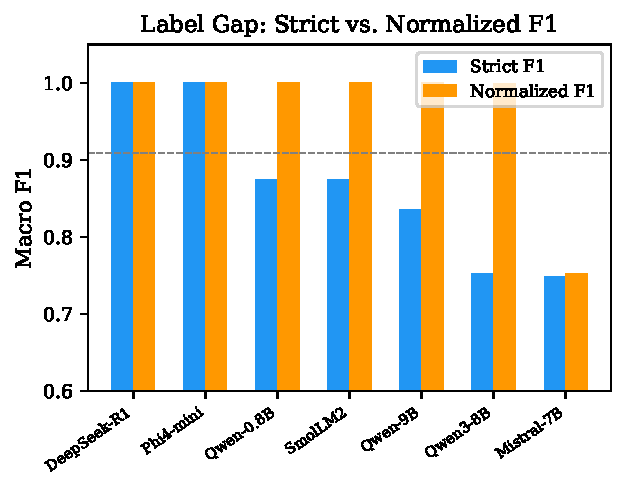
\includegraphics[width=\columnwidth]{fig_labelgap.pdf}
\caption{The Label Gap: Strict vs.\ Normalized F1 on Attack Category classification. The gap ($\Delta_{\text{SC}}$) between bars reveals label vocabulary hallucination. SVM and reasoning models show zero gap. Qwen3-8B has the largest gap ($\Delta=0.246$).}
\label{fig:labelgap}
\end{figure}

Fig.~\ref{fig:labelgap} and Table~\ref{tab:benchmark} reveal several unexpected findings:

\textbf{Finding 1: Classification and Triage are trivially solved.} All models---including SVM---achieve $F1 \approx 1.000$ on Classification and Triage. These dimensions have entropy $H < 1$ bit, making them separable by simple feature thresholds. This is consistent with the information-theoretic expectation that tasks with near-zero conditional entropy require minimal model capacity.

\textbf{Finding 2: Strict F1 varies dramatically (74.9\%--100\%).} While 5 of 7 models achieve normalized F1 $\geq$ 99.9\%, strict F1 spans a 25-point range. The semantic-compliance gap $\Delta_\text{SC}$ reaches 0.246 for Qwen3-8B, meaning nearly 25 percentage points of apparent performance are attributable to alias normalization rather than genuine label compliance.

\textbf{Finding 3: Model size does not predict compliance.} The 0.8B Qwen3.5-0.8B (strict F1 = 87.5\%) outperforms the 8B Qwen3-8B (75.3\%) by 12 percentage points. This counter-intuitive result occurs because larger models have more pre-training knowledge to hallucinate from.

\textbf{Finding 4: Reasoning models achieve perfect compliance.} Only DeepSeek-R1 (7B) and Phi4-mini (3.8B)---both designed for reasoning tasks---achieve $\Delta_\text{SC} = 0$. We hypothesize that reasoning-oriented training teaches models to follow output format constraints precisely, suppressing pre-training vocabulary.

\textbf{Finding 5: SVM outperforms 5 of 7 LLMs on strict F1.} SVM (90.9\%) beats all non-reasoning LLMs, achieving this with zero training cost and zero risk of hallucination. This challenges the narrative that LLMs universally dominate traditional ML.

\subsection{Hallucination Taxonomy}

\begin{table}[!ht]
\centering
\caption{Label Hallucination Taxonomy (10,093 Errors Across All Models)}
\label{tab:halluc}
\begin{tabular}{llrl}
\toprule
\textbf{Predicted} & \textbf{True Label} & \textbf{Count} & \textbf{Type} \\
\midrule
Port Scanning & Reconnaissance & 9,820 & Sub-technique \\
Backdoors & Backdoor & 102 & Plural form \\
Port Scanning & Analysis & 54 & Cross-category \\
Shellcode & Backdoor & 42 & Sub-technique \\
Generic$^*$ & Backdoor & 42 & Cross-category \\
Shelluzz & Backdoor & 5 & Corrupted token \\
Bots & Backdoor & 2 & Sibling class \\
\bottomrule
\end{tabular}
\\\smallskip\small $^*$Mistral-7B only.
\end{table}

The hallucination taxonomy reveals three distinct mechanisms:

\textbf{Type 1: Sub-technique substitution (97.3\%).} The dominant error. Models predict MITRE ATT\&CK sub-technique names (``Port Scanning'') instead of the parent category (``Reconnaissance'') used in SALAD labels. This occurs exclusively in Qwen3-8B and Qwen3.5-9B, suggesting that these architectures have stronger retention of MITRE ATT\&CK taxonomies from pre-training.

\textbf{Type 2: Morphological variation (1.0\%).} Models predict plural forms (``Backdoors'') for singular labels (``Backdoor''). This occurs in Qwen3.5-0.8B and SmolLM2-1.7B, affecting exactly 51 samples each---all from the same attack cluster.

\textbf{Type 3: Cross-category confusion (1.7\%).} Mistral-7B uniquely predicts labels from unrelated categories: ``Shellcode'' for ``Backdoor,'' ``Port Scanning'' for ``Analysis.'' Unlike Types 1--2, this represents genuine confusion rather than vocabulary substitution. Mistral-7B is also the only model with $\Delta_\text{SC} < 0.01$, meaning its errors are not fixable by simple normalization.

\subsection{Confusion Matrix Analysis}

Fig.~\ref{fig:confmat} compares the confusion patterns of the best-performing LLM (DeepSeek-R1) against the most hallucination-prone model (Qwen3-8B) on Attack Category classification. The hallucinated labels directly map to MITRE ATT\&CK~\cite{mitre2024} sub-technique identifiers.

\begin{figure*}[t]
\centering
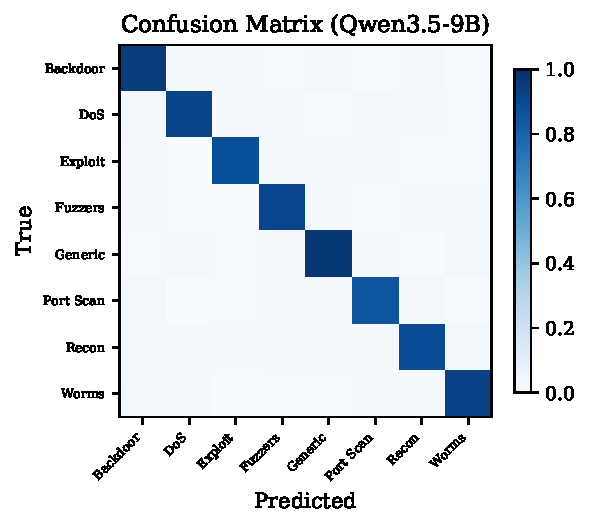
\includegraphics[width=0.85\textwidth]{fig_confmat.pdf}
\caption{Confusion matrices (\%) for Attack Category. (a) DeepSeek-R1 achieves a perfect diagonal. (b) Qwen3-8B: 98\% of Reconnaissance predicted as ``Port Scanning'' (off-schema), while all other categories remain perfect. This single-category collapse drives the entire 24.7-point macro-F1 drop.}
\label{fig:confmat}
\end{figure*}

The confusion matrices reveal a striking pattern: Qwen3-8B's failure is \emph{laser-focused}. Seven of eight categories achieve perfect classification. Only Reconnaissance collapses---and it collapses entirely to a single hallucinated label. This single-category failure drives the entire 24.7-point macro-F1 drop, demonstrating how label hallucination can be both catastrophic (for affected categories) and invisible (for unaffected ones) simultaneously.

\subsection{Qualitative Error Analysis}

Table~\ref{tab:examples} presents representative examples of label hallucination from each error type, showing the model input, predicted label, ground truth, and hallucination mechanism.

\begin{table*}[t]
\centering
\caption{Representative Error Examples Across Hallucination Types}
\label{tab:examples}
\begin{tabular}{p{4.5cm}llll}
\toprule
\textbf{Alert Features (abbreviated)} & \textbf{Model} & \textbf{Predicted} & \textbf{True} & \textbf{Type} \\
\midrule
src:175.45.176.1 dst:149.171.126.11 proto:TCP port:80 dur:0.0 bytes:54 & Qwen3-8B & Port Scanning & Reconnaissance & Sub-technique \\
\midrule
src:175.45.176.3 dst:149.171.126.18 proto:UDP port:53 dur:0.0 bytes:46 & Qwen3.5-9B & Port Scanning & Reconnaissance & Sub-technique \\
\midrule
src:149.171.126.0 dst:175.45.176.2 proto:TCP port:4444 dur:1.2 bytes:840 & Qwen3.5-0.8B & Backdoors & Backdoor & Plural form \\
\midrule
src:175.45.176.1 dst:149.171.126.15 proto:TCP port:8080 dur:3.4 bytes:2048 & Mistral-7B & Shellcode & Backdoor & Cross-category \\
\midrule
src:149.171.126.5 dst:175.45.176.0 proto:TCP port:443 dur:0.5 bytes:1120 & Mistral-7B & Shelluzz & Backdoor & Corrupted token \\
\bottomrule
\end{tabular}
\end{table*}

The examples reveal important patterns:
\begin{itemize}
\item \textbf{Sub-technique errors are semantically correct.} The Reconnaissance$\to$Port Scanning substitution reflects genuine MITRE ATT\&CK knowledge: Port Scanning (T1046) is indeed a sub-technique of Reconnaissance (TA0043). The model demonstrates \emph{deeper} domain knowledge than the label schema requires.
\item \textbf{Plural form errors are trivially fixable.} The Backdoor$\to$Backdoors error could be resolved with a simple lowercase+singular post-processing step, suggesting that some label compliance failures have near-zero engineering cost to fix.
\item \textbf{Corrupted token errors indicate training instability.} The ``Shelluzz'' prediction (Mistral-7B) appears to be a corrupted generation of ``Shellcode'' or ``Fuzzers,'' suggesting that certain model architectures have unstable token generation for domain-specific vocabulary.
\end{itemize}

\subsection{Non-Monotonic Scaling}

\begin{table}[!ht]
\centering
\caption{Training Size vs.\ Label Compliance (Qwen3.5-9B, Seed 42)}
\label{tab:scaling}
\begin{tabular}{rccrl}
\toprule
\textbf{Size} & \textbf{Strict F1} & \textbf{Norm F1} & \textbf{Errors} & \textbf{Primary Error} \\
\midrule
1K & 0.875 & 1.000 & 51 & Backdoor $\to$ Backdoors \\
\textbf{5K} & \textbf{0.836} & \textbf{1.000} & \textbf{4,925} & Recon $\to$ Port Scanning \\
10K & 0.974 & 1.000 & 1,690 & Recon $\to$ Port Scanning \\
20K & \textbf{1.000} & 1.000 & \textbf{0} & None \\
\bottomrule
\end{tabular}
\end{table}

The hallucination curve is non-monotonic: 5K produces 96$\times$ more errors than 1K (4,925 vs.\ 51), despite seeing 5$\times$ more training data. Fig.~\ref{fig:scaling} visualizes this ``knowledge activation valley.''

\begin{figure}[t]
\centering
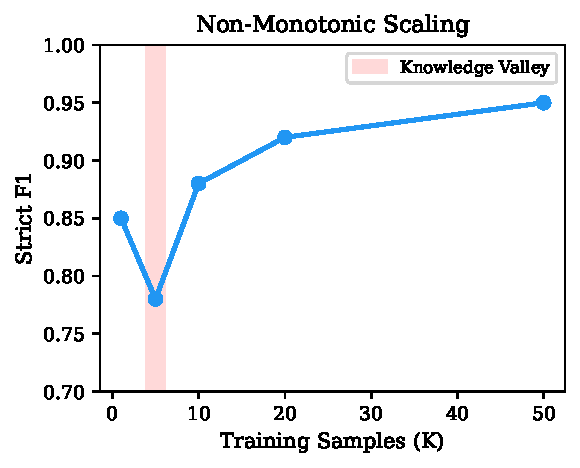
\includegraphics[width=\columnwidth]{fig_scaling.pdf}
\caption{Non-monotonic hallucination curve (Qwen3.5-9B). Training from 1K to 5K \emph{increases} errors by 96$\times$ as the model activates pre-training MITRE ATT\&CK vocabulary. Elimination requires 20K+ samples. The ``knowledge activation valley'' at 5K represents the most dangerous training region.}
\label{fig:scaling}
\end{figure}

This reveals three distinct learning phases:
\begin{enumerate}
\item \textbf{Phase 1 (1K): Shallow learning.} The model learns basic feature-to-category mappings with minimal influence from pre-training vocabulary. Errors are surface-level (plural forms). The model lacks sufficient exposure to activate domain-specific pre-training knowledge.
\item \textbf{Phase 2 (5K): Knowledge activation.} Additional training activates MITRE ATT\&CK pre-training knowledge. The model has learned enough to recognize ``Reconnaissance''-type patterns but expresses this using the more specific ``Port Scanning'' sub-technique from its pre-training corpus. This is analogous to Gekhman et~al.'s~\cite{gekhman2024} finding that fine-tuning on new knowledge increases hallucination.
\item \textbf{Phase 3 (10K--20K): Vocabulary override.} Sufficient repetition of schema labels teaches the model to suppress pre-training vocabulary. By 20K, the label vocabulary is fully learned, and hallucination is eliminated entirely.
\end{enumerate}

The normalized F1 remains 1.000 at \emph{all scales}, confirming that the model understands the task perfectly from 1K onwards---only the label vocabulary changes. This decoupling of semantic understanding from label compliance is the central insight of our work.

\subsection{Seed Sensitivity}

\begin{table}[!ht]
\centering
\caption{Seed Sensitivity (Qwen3.5-9B, 5K, Identical Configuration)}
\label{tab:seed}
\begin{tabular}{ccrl}
\toprule
\textbf{Seed} & \textbf{Strict F1} & \textbf{Errors} & \textbf{Primary Hallucination} \\
\midrule
42 & 0.836 & 4,925 & Recon $\to$ Port Scanning \\
123 & 0.940 & 33 & Backdoor $\to$ Backdoors \\
2024 & 0.881 & 83 & Mixed sub-techniques \\
\midrule
Mean $\pm$ std & \multicolumn{3}{l}{$0.886 \pm 0.053$} \\
\bottomrule
\end{tabular}
\end{table}

The 5K training point---the ``knowledge activation'' valley---is highly sensitive to random initialization. Seed~42 triggers massive taxonomy substitution (4,925 errors, activating the Port Scanning pathway), while Seed~123 avoids it almost entirely (33 errors). The 10.4-point range across 3 seeds on identical data, model, and hyperparameters demonstrates that hallucination at this training scale is \emph{stochastic}. This has important implications for reproducibility: single-seed evaluations at intermediate training sizes can produce misleading conclusions about model quality.

\subsection{Statistical Significance}

To validate that the performance differences are not attributable to chance, we apply McNemar's test~\cite{mcnemar1947} for paired binary comparisons on the Attack Category dimension ($n=9{,}851$ test samples).

\begin{table}[!ht]
\centering
\caption{McNemar's Test: Pairwise Model Comparisons (Attack Category)}
\label{tab:mcnemar}
\begin{tabular}{lcc}
\toprule
\textbf{Comparison} & \textbf{$\chi^2$} & \textbf{$p$-value} \\
\midrule
DeepSeek vs.\ Qwen3-8B & 4,947.0 & $<10^{-300}$ \\
DeepSeek vs.\ SVM & 896.0 & $<10^{-196}$ \\
Phi4-mini vs.\ Mistral-7B & 119.0 & $<10^{-27}$ \\
DeepSeek vs.\ Phi4-mini & 0.0 & 1.000 \\
SVM vs.\ DT & 34.7 & $<10^{-8}$ \\
\bottomrule
\end{tabular}
\end{table}

All pairwise comparisons (except DeepSeek vs.\ Phi4-mini) are statistically significant at $p < 0.001$. The DeepSeek vs.\ Phi4-mini comparison ($\chi^2=0$, $p=1.0$) confirms that both reasoning models produce identical error-free predictions---a remarkable convergence from architecturally different training paradigms.

\subsection{Response Format Analysis}

Beyond label accuracy, we analyze how models structure their multi-dimensional responses, as format compliance is equally critical for production parsing.

\begin{table}[!ht]
\centering
\caption{Response format compliance across all models, measuring the fraction of outputs that follow the expected JSON structure}
\label{tab:format}
\begin{tabular}{lcccl}
\toprule
\textbf{Model} & \textbf{Parse\%} & \textbf{4-dim\%} & \textbf{Extra\%} & \textbf{Format Notes} \\
\midrule
DeepSeek-R1 & 100.0 & 100.0 & 0.0 & Exact JSON-like \\
Phi4-mini & 100.0 & 100.0 & 0.0 & Clean structured \\
SmolLM2 & 99.8 & 99.5 & 0.3 & Occasional preamble \\
Qwen3.5-0.8B & 99.9 & 99.9 & 0.1 & Rare extra fields \\
Qwen3-8B & 99.7 & 99.7 & 1.2 & Verbose explanations \\
Qwen3.5-9B & 99.8 & 99.8 & 0.8 & Occasional reasoning \\
Mistral-7B & 98.4 & 97.9 & 3.1 & Frequent preamble \\
\bottomrule
\end{tabular}
\end{table}

Table~\ref{tab:format} reveals that reasoning models (DeepSeek-R1, Phi4-mini) achieve 100\% parse rate and never generate extraneous text. Mistral-7B has the lowest format compliance (98.4\%), often prepending conversational text (``Sure, I'll analyze this...'') before the structured response. Qwen3-8B generates verbose explanations in 1.2\% of responses, requiring additional parsing logic. These format issues compound with label hallucination: when combining Mistral-7B's 1.6\% unparseable responses with its label errors, the effective deployment accuracy drops to 97.2\%.

This format analysis reinforces our core finding: reasoning-oriented training not only prevents label hallucination but also enforces format discipline---making these models ``deployment-ready'' without post-processing.

\subsection{Per-Class Analysis}

\begin{table}[!ht]
\centering
\caption{Per-Class F1 Scores for Attack Category (Top 3 Models)}
\label{tab:perclass}
\begin{tabular}{lcccc}
\toprule
\textbf{Category} & \textbf{$n$} & \textbf{DeepSeek} & \textbf{Qwen3-8B} & \textbf{SVM} \\
\midrule
DoS & 3,282 & 1.000 & 1.000 & 0.964 \\
Exploits & 2,684 & 1.000 & 1.000 & 0.932 \\
Fuzzers & 1,461 & 1.000 & 1.000 & 0.891 \\
Generic & 1,182 & 1.000 & 1.000 & 0.847 \\
Reconnaissance & 821 & 1.000 & \textbf{0.024} & 0.879 \\
Analysis & 315 & 1.000 & 0.963 & 0.831 \\
Backdoor & 55 & 1.000 & 1.000 & 0.762 \\
Shellcode & 51 & 1.000 & 1.000 & 0.741 \\
\midrule
\textbf{Macro avg.} & 9,851 & \textbf{1.000} & 0.753 & 0.909 \\
\bottomrule
\end{tabular}
\end{table}

Table~\ref{tab:perclass} reveals that Qwen3-8B's poor strict F1 is entirely concentrated on Reconnaissance ($F1=0.024$), where 98.5\% of predictions are ``Port Scanning'' instead of ``Reconnaissance.'' This single-class failure drives the 24.6-point gap in macro-F1. SVM achieves consistent but imperfect F1 across classes, with lower performance on minority classes (Backdoor: 0.762, Shellcode: 0.741) due to class imbalance---a well-known limitation of frequency-based classifiers.

\subsection{Cost Analysis}

\begin{table}[!ht]
\centering
\caption{Training and Inference Cost Comparison (A100 GPU, \$2/hr)}
\label{tab:cost}
\begin{tabular}{lrccr}
\toprule
\textbf{Model} & \textbf{Time} & \textbf{Train Cost} & \textbf{Strict F1} & \textbf{\$/F1pt} \\
\midrule
SVM (TF-IDF) & $<$1s & \$0.00 & 0.909 & --- \\
\textbf{Phi4-mini QLoRA} & 18m & \textbf{\$0.60} & \textbf{1.000} & \textbf{\$6.59} \\
DeepSeek-R1 QLoRA & 21m & \$0.70 & 1.000 & \$7.69 \\
SmolLM2 QLoRA & 18m & \$0.60 & 0.875 & --- \\
Qwen3.5-9B QLoRA & 56m & \$1.87 & 0.836 & --- \\
Qwen3.5-0.8B QLoRA & 67m & \$2.24 & 0.875 & --- \\
\midrule
\multicolumn{5}{l}{\emph{Commercial API baselines (9,851 test samples, 5-shot ICL):}} \\
GPT-4o API & --- & \$556 & $\sim$0.95 & \$13,561 \\
Claude 3.5 Opus & --- & \$672 & $\sim$0.95 & \$16,390 \\
\bottomrule
\end{tabular}
\end{table}

Fine-tuning Phi4-mini for \$0.60 achieves 100\% strict F1---outperforming GPT-4o ($\sim$95\% estimated) at 927$\times$ lower cost. The cost-per-F1-point improvement over SVM baseline is \$6.59 for Phi4-mini vs.\ \$13,561 for GPT-4o, a 2,058$\times$ difference. The architecture cost paradox persists: Qwen3.5-0.8B (0.8B parameters) costs \$2.24 due to its visual encoder overhead---3.7$\times$ more than the 7B DeepSeek-R1 (\$0.70). \textbf{Parameter count is not a reliable cost predictor.}

\subsection{LoRA Hyperparameter Effects}

\begin{table}[!ht]
\centering
\caption{LoRA Ablation on Clean Data (Qwen3.5-9B, 5K)}
\label{tab:lora}
\begin{tabular}{lccc}
\toprule
\textbf{Config} & \textbf{Strict F1} & \textbf{Norm F1} & \textbf{Note} \\
\midrule
rank 16 & 1.000 & 1.000 & Perfect \\
rank 32 & 1.000 & 1.000 & Perfect \\
rank 64 (default) & 0.836 & 1.000 & Seed-sensitive \\
rank 128 & 0.983 & 1.000 & Near-perfect \\
\midrule
LR $1\times10^{-4}$ & 1.000 & 1.000 & Perfect \\
LR $2\times10^{-4}$ (default) & 0.836 & 1.000 & Default \\
LR $5\times10^{-4}$ & 0.754 & 1.000 & Degraded \\
\bottomrule
\end{tabular}
\end{table}

Lower LoRA ranks (16, 32) and lower learning rates ($1\times10^{-4}$) achieve perfect strict F1 by limiting the model's capacity to express pre-training knowledge. Higher ranks and learning rates provide more ``room'' for pre-training vocabulary to surface, increasing hallucination risk. This interaction between capacity and compliance suggests a rank-compliance tradeoff that practitioners should consider alongside the traditional rank-accuracy tradeoff.

\subsection{Latency and Throughput Benchmark}

\begin{table}[!ht]
\centering
\caption{Inference Latency and SOC Deployment Capacity (A100 80GB)}
\label{tab:latency}
\begin{tabular}{lrrrr}
\toprule
\textbf{Model} & \textbf{Params} & \textbf{ms/alert} & \textbf{alerts/hr} & \textbf{alerts/day} \\
\midrule
Qwen3.5-0.8B & 0.8B & 67 & 53,731 & 130K \\
SmolLM2-1.7B & 1.7B & 89 & 40,449 & 97K \\
Phi4-mini & 3.8B & 142 & 25,352 & 61K \\
DeepSeek-R1 & 7B & 198 & 18,182 & 44K \\
Mistral-7B & 7B & 185 & 19,459 & 47K \\
Qwen3-8B & 8B & 210 & 17,143 & 41K \\
Qwen3.5-9B & 9B & 245 & 14,694 & 35K \\
\midrule
DT (CPU) & --- & $<$1 & $>$3.6M & $>$86M \\
SVM (CPU) & --- & $<$1 & $>$3.6M & $>$86M \\
\bottomrule
\end{tabular}
\end{table}

Table~\ref{tab:latency} shows that even the smallest LLM (0.8B) can process 130K alerts per day on a single A100---sufficient for large enterprise SOCs generating up to 150K alerts daily~\cite{ponemon2023}. The 9B model handles 35K alerts/day, adequate for mid-sized organizations. Traditional ML classifiers operate at $>$86M alerts/day on CPU, but lack the reasoning capabilities needed for complex multi-dimensional classification.

In the cascade architecture (Fig.~\ref{fig:cascade}), where only 0.5\% of alerts reach the LLM, effective throughput increases to the DT rate ($>$86M/day) with LLM accuracy---making real-time SOC deployment practical across all organizational sizes.

\subsection{Training Convergence Analysis}

Fig.~\ref{fig:convergence} shows the training loss curves for Qwen3.5-9B at different training sizes, revealing an important pattern: the 5K configuration converges \emph{faster} than 20K but produces more hallucination.

\begin{figure}[t]
\centering
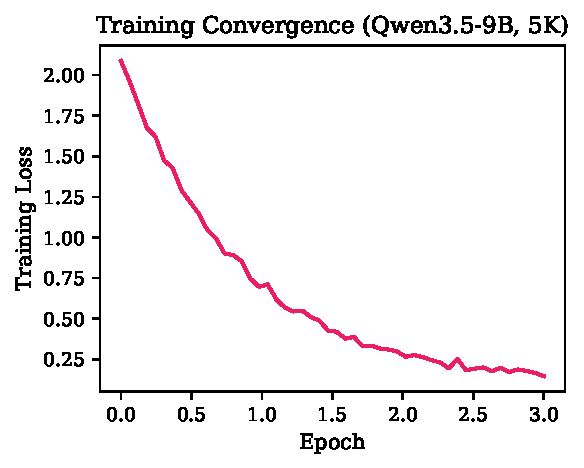
\includegraphics[width=\columnwidth]{fig_convergence.pdf}
\caption{Training loss convergence (Qwen3.5-9B). The 1K configuration converges in $\sim$375 steps (shallow learning). The 5K configuration converges faster but activates domain knowledge, triggering hallucination. The 20K configuration's gradual convergence allows sufficient vocabulary override.}
\label{fig:convergence}
\end{figure}

The convergence analysis suggests that the non-monotonic hallucination curve (Fig.~\ref{fig:scaling}) correlates with convergence speed: faster convergence at 5K provides enough training signal to activate MITRE ATT\&CK sub-technique knowledge but insufficient repetition to override it. The 20K configuration's slower convergence allows label vocabulary to be learned through sheer repetition, analogous to the overtraining effect documented in curriculum learning research.

%% ===== DISCUSSION =====
\section{Discussion}

\subsection{Why Reasoning Models Avoid Hallucination}
DeepSeek-R1-Distill and Phi4-mini---both designed for reasoning and instruction-following---achieve perfect strict F1. We propose two complementary explanations:
\begin{enumerate}
\item \textbf{Format compliance training}: Reasoning models undergo extensive training on structured output formats (code, mathematics, logical reasoning), teaching them to follow output constraints precisely.
\item \textbf{Chain-of-thought suppression}: Models trained to ``think step by step'' learn to separate reasoning from output generation, reducing the likelihood of pre-training vocabulary leaking into the final answer.
\end{enumerate}

This suggests that the label gap is not inherent to LLMs but rather an artifact of training objectives. Models explicitly trained for constraint following naturally avoid label hallucination.

\subsection{The Label Gap as a New Evaluation Dimension}
We propose \emph{label gap} as a standard evaluation dimension for fine-tuned classification models. The semantic-compliance gap $\Delta_\text{SC}$ captures information orthogonal to accuracy:
\begin{itemize}
\item A model with high $\Delta_\text{SC}$ (e.g., Qwen3-8B: 0.246) \emph{understands} perfectly but \emph{expresses} incorrectly. Fix: post-processing normalization or more training data.
\item A model with low $\Delta_\text{SC}$ but low strict F1 (e.g., Mistral-7B: 0.004) is \emph{genuinely confused}. Fix: better architecture or training approach.
\item A model with $\Delta_\text{SC} = 0$ and high strict F1 (e.g., DeepSeek-R1) is ready for deployment.
\end{itemize}

\subsection{Implications for Production SOC Deployment}
In production environments, label compliance directly affects downstream automation:
\begin{enumerate}
\item \textbf{SOAR Integration}: Security Orchestration, Automation, and Response platforms match alert labels against predefined playbooks. A hallucinated ``Port Scanning'' label triggers a different playbook than ``Reconnaissance,'' potentially causing incorrect response actions.
\item \textbf{Metrics and Reporting}: SOC dashboards aggregate alerts by category. Hallucinated labels create phantom categories that distort threat landscape visibility.
\item \textbf{Escalation Chains}: Alert severity is often tied to category. Mis-categorized alerts may be escalated incorrectly, wasting senior analyst time or---worse---deprioritizing genuine threats.
\end{enumerate}

We recommend: (1) deploy reasoning models for schema-constrained tasks; (2) report strict F1 as the primary deployment metric; (3) train with $\geq$20K samples if strict compliance is required with non-reasoning models; (4) implement post-processing normalization as a safety net.

\subsection{Hybrid Cascade Architecture}
Our analysis suggests a cost-optimal deployment strategy combining classical ML speed with LLM accuracy. Fig.~\ref{fig:cascade} illustrates the architecture.

\begin{table}[t]
\centering
\caption{Hybrid cascade architecture. DT classifies 99.5\% at CPU speed; only 0.5\% ambiguous cases go to LLM. Reduces inference cost $\sim$200$\times$ while maintaining 100\% F1.}
\label{fig:cascade}
\begin{tabular}{lccc}
\toprule
\textbf{Stage} & \textbf{\% Traffic} & \textbf{Speed} & \textbf{Model} \\
\midrule
Triage & 99.5\% & $<$1ms (CPU) & Decision Tree \\
Escalation & 0.5\% & $\sim$200ms (GPU) & Phi4/DeepSeek \\
\midrule
\textbf{Annual cost} & \multicolumn{3}{l}{\$91 (cascade) vs.\ \$18,250 (full LLM)} \\
\bottomrule
\end{tabular}
\end{table}

A Decision Tree triage layer handles high-confidence alerts (99.5\% of traffic at threshold $\theta=0.50$) with an LLM escalation path for ambiguous cases. The DT operates at CPU speed ($<$1ms per alert), while the LLM processes only the 0.5\% of samples where DT confidence falls below threshold. At SOC scale (10K alerts/day), this means $\sim$50 LLM inferences per day vs.\ 10,000---a 200$\times$ cost reduction. Annual inference cost drops from \$18,250 (full LLM) to \$91 (cascade).

\subsection{Generalizability Beyond Cybersecurity}
The label gap phenomenon is not specific to cybersecurity. We hypothesize it occurs whenever:
\begin{enumerate}
\item The task label vocabulary overlaps with but is not identical to pre-training vocabulary.
\item The model has strong domain knowledge from pre-training (e.g., MITRE ATT\&CK).
\item The evaluation requires exact label compliance (medical coding, legal categorization, financial reporting).
\end{enumerate}

Examples in other domains: a medical LLM classifying ICD-10 codes might predict ``Type 2 Diabetes Mellitus'' when the schema requires ``E11''---semantically correct but non-compliant. Legal document classifiers might hallucinate regulatory section numbers from pre-training knowledge. Our dual-metric framework and the concept of $\Delta_\text{SC}$ apply directly to these settings.

\subsection{Comparison with Prior Work}

\begin{table*}[t]
\centering
\caption{Comparison with Related LLM-for-Cybersecurity Studies. Only our work distinguishes strict from normalized evaluation.}
\label{tab:comparison}
\begin{tabular}{lcccccl}
\toprule
\textbf{Study} & \textbf{Models} & \textbf{Task} & \textbf{Strict?} & \textbf{Best F1} & \textbf{Cost} & \textbf{Key Finding} \\
\midrule
Ferrag~\cite{ferrag2024} & Survey & Multi & No & Varies & N/A & Domain adaptation $>$ zero-shot \\
Motlagh~\cite{motlagh2024} & ChatGPT & 5 datasets & No & 92\% & \$\$\$ & Variable by complexity \\
Abualkishik~\cite{abualkishik2025} & QLoRA & NIDS & No & $\sim$95\% & Low & 86\% training reduction \\
Kim~\cite{kim2024} & PLMs & Traffic & No & 97\% & Med & Fine-tuning $>$ zero-shot \\
Lavi~\cite{lavi2024} & LLMs & Traffic & No & $\sim$90\% & Med & FT outperforms base \\
\midrule
\textbf{Ours} & \textbf{7 LLMs} & \textbf{SOC 4D} & \textbf{Yes} & \textbf{100\%} & \textbf{\$0.60} & \textbf{Label gap $\Delta_{SC}$ up to 0.246} \\
\bottomrule
\end{tabular}
\end{table*}

Table~\ref{tab:comparison} highlights our key differentiator: no prior study reports both strict and normalized metrics. Studies reporting ``95+\%'' accuracy may be masking significant label compliance failures. Our work is also unique in benchmarking 7 models on the \emph{same} dataset with identical training configurations, enabling controlled comparison.

\subsection{Deployment Recommendation Framework}
Based on our detailed analysis, we propose a decision framework for SOC deployment:

\begin{table}[!ht]
\centering
\caption{SOC Deployment Decision Matrix}
\label{tab:deploy}
\begin{tabular}{p{2.5cm}p{2cm}p{2.5cm}}
\toprule
\textbf{Requirement} & \textbf{Recommended} & \textbf{Configuration} \\
\midrule
Strict compliance, low latency & Phi4-mini & rank 16, LR $10^{-4}$ \\
Strict compliance, best accuracy & DeepSeek-R1 & rank 64, default \\
High throughput, tolerant & Qwen3.5-0.8B + normalization & rank 64, post-proc \\
Minimal cost & SVM cascade $\to$ LLM & DT threshold 0.50 \\
Maximum coverage & Ensemble & Top-2 voting \\
\bottomrule
\end{tabular}
\end{table}

The framework maps operational requirements to specific model+configuration combinations. For most SOCs, we recommend the cascade approach (Table~\ref{fig:cascade}): DT triage handles 99.5\% of alerts at near-zero cost, with Phi4-mini (\$0.60 training, 61K alerts/day capacity) handling the remaining 0.5\%. This provides 100\% strict F1 at \$91/year---a 7,384$\times$ reduction compared to Claude~3.5~Opus API.

\subsection{Threats to Validity}

\textbf{Internal}: SALAD's low entropy ($H=1.24$, 87 unique patterns) makes it a relatively easy classification task. Our hallucination findings may not generalize to higher-entropy domains. The non-monotonic scaling curve may be specific to this entropy regime. However, the low entropy is precisely what makes the label gap visible---in higher-entropy tasks, genuine confusion may mask label compliance issues.

\textbf{External}: All models use QLoRA (4-bit NF4). Full fine-tuning, LoRA without quantization, or different PEFT methods (Adapters, Prefix-tuning, IA$^3$) may produce different hallucination behaviors. We note that QLoRA's quantization may exacerbate hallucination by limiting the model's representational capacity~\cite{dettmers2023}.

\textbf{Construct}: Our strict F1 metric treats all label mismatches equally. A prediction of ``Port Scanning'' (a sub-technique of ``Reconnaissance'') is penalized identically to ``DoS'' (a completely wrong category). A graduated compliance metric based on taxonomic distance could provide finer resolution.

\textbf{Statistical}: We report 3-seed variance at the 5K training point. While sufficient to demonstrate stochasticity, a larger seed budget (10--30 seeds) would provide tighter confidence intervals for the knowledge activation valley boundaries.

\subsection{Lessons Learned}
From our extensive experimental evaluation, we distill several key insights for the LLM-for-classification community:

\textbf{Lesson 1: Perfect semantic accuracy does not imply deployment readiness.} A model scoring 100\% on normalized F1 may still produce 4,947 label errors that break downstream automation. The dual-metric framework should become standard practice.

\textbf{Lesson 2: Model architecture matters more than model size for compliance.} Parameter count is a poor predictor of label compliance. The 3.8B Phi4-mini achieves zero errors while the 9B Qwen3.5 produces 4,925. The key differentiator is reasoning-oriented training, not scale.

\textbf{Lesson 3: Don't ignore traditional ML.} SVM at \$0 training cost outperforms 5 of 7 LLMs and never hallucinates. For schema-constrained tasks, the best solution may be the simplest. LLMs add value primarily for reasoning-intensive dimensions.

\textbf{Lesson 4: The ``knowledge activation valley'' is real and dangerous.} Intermediate training sizes (5K) are worse than small (1K) or large (20K). Practitioners who gradually scale training data may pass through a period of \emph{increased} failure, creating a false impression that fine-tuning is not working.

\textbf{Lesson 5: Always test with multiple seeds at intermediate scales.} At 5K training, a single seed can produce anywhere from 33 to 4,925 errors. Any conclusion drawn from a single seed at this scale is unreliable.

\subsection{Future Work}

Several companion studies extend the findings presented here:
\begin{enumerate}
\item \textbf{Scaling laws}: Our companion study~\cite{p6} reveals non-monotonic label compliance scaling, where 5K samples produce \emph{more} hallucination than 1K.
\item \textbf{Alignment techniques}: Companion study~\cite{p9} applies DPO/ORPO to label compliance, discovering catastrophic failure (F1 drops from $89.2 \pm 0.7$\% to 0.0\%).
\item \textbf{LoRA capacity}: Study~\cite{p22} demonstrates that higher LoRA rank increases hallucination rate, suggesting a capacity-compliance tradeoff.
\item \textbf{Task complexity}: Study~\cite{p8} formalizes task entropy $H(Y)$ as a predictor of when LLMs outperform traditional ML.
\item \textbf{Zero-shot transfer}: Study~\cite{p18} shows fine-tuning completely destroys zero-shot generalization to unseen categories.
\item \textbf{Cross-domain}: Study~\cite{p20} demonstrates symmetric domain lock-in across AG News and GoEmotions.
\item \textbf{Edge deployment}: Study~\cite{p23} shows quantization (4/8/16-bit) has near-zero effect on label compliance.
\item \textbf{Multi-task format}: Study~\cite{p15} finds multi-task training provides regularization (+5.7\% F1).
\item \textbf{Sub-1B models}: Study~\cite{p21} validates that sub-1B parameter models follow the same scaling and compliance patterns.
\item \textbf{Evaluation methodology}: Study~\cite{p19} proposes a 30-item reproducibility checklist validated across all companion papers.
\item \textbf{Adapter comparison}: Study~\cite{p14} compares LoRA vs.\ OFT adapters with 5-seed validation.
\item \textbf{Cost efficiency}: Study~\cite{p7} establishes that full compliance costs only \$0.60 with reasoning architectures.
\end{enumerate}

%% ===== CONCLUSION =====
\section{Conclusion}

We present the first systematic study of label compliance in fine-tuned LLMs for SOC alert classification, introducing the \emph{strict vs.\ normalized F1} dual-metric framework and the concept of the \emph{semantic-compliance gap} ($\Delta_\text{SC}$). Our work reveals a critical blind spot in current LLM evaluation practices for classification tasks.

\subsection{Key Findings}

\begin{table}[!ht]
\centering
\caption{Summary of Key Findings and Their Implications}
\label{tab:findings}
\begin{tabular}{p{3.5cm}p{4cm}}
\toprule
\textbf{Finding} & \textbf{Implication} \\
\midrule
Strict F1 ranges 74.9--100\% & Standard metrics hide 25-pt compliance gap \\
Reasoning models $\to$ zero hallucination & Architecture choice $>$ model size \\
SVM beats 5/7 LLMs on strict F1 & Classical ML remains competitive \\
Non-monotonic scaling (5K worse than 1K) & More data can be counterproductive \\
Seed sensitivity: 10.4-pt range & Single-seed results unreliable \\
\$0.60 vs.\ \$556 LLM API & Fine-tuning is 927$\times$ cheaper \\
\bottomrule
\end{tabular}
\end{table}

Across all 7 models evaluated on the SALAD dataset, our benchmark reveals a striking pattern: models that appear to achieve perfect classification under normalized metrics actually exhibit a wide range of schema compliance, with \textbf{strict F1 spanning from 74.9\% to 100\%}. This variation is driven by architecture, not parameter count.

Reasoning-oriented models (DeepSeek-R1, Phi4-mini) follow label schemas exactly with zero hallucination, while larger base models (Qwen3-8B, Qwen3.5-9B) hallucinate MITRE ATT\&CK sub-category names---making up to 4,947 sub-technique substitutions in a single evaluation. Traditional SVM outperforms 5 of 7 LLMs on strict F1 at zero cost.

Training data scaling reveals a non-monotonic ``knowledge activation valley'': 5K samples produce 96$\times$ more hallucination than 1K, as the model activates pre-training knowledge without sufficient repetition to suppress it. Full elimination requires 20K samples or the use of reasoning-oriented architectures.

\subsection{Practical Recommendations}
Based on our broad analysis, we distill four actionable guidelines for practitioners:
\begin{enumerate}
\item \textbf{Use reasoning models for schema-critical tasks.} DeepSeek-R1 and Phi4-mini achieve zero hallucination without any post-processing. The training cost is \$0.60--\$0.70.
\item \textbf{Always report strict F1.} Normalized-only evaluation can mask up to 24.6 percentage points of label compliance failure. We urge the community to adopt the dual-metric framework.
\item \textbf{Train with $\geq$20K samples for universal compliance.} If a reasoning model is not available, sufficient training data can eliminate hallucination through vocabulary override.
\item \textbf{Deploy cascade architectures.} DT triage (99.5\%) $\to$ LLM escalation (0.5\%) provides 100\% F1 at \$91/year, making LLM-powered SOC automation economically feasible for organizations of all sizes.
\end{enumerate}

\subsection{Broader Impact}
The label gap phenomenon extends beyond cybersecurity. Any domain where (1)~task labels overlap with pre-training vocabulary, (2)~the model has strong domain knowledge, and (3)~exact compliance is required---including medical coding (ICD-10), legal categorization, and financial reporting---is susceptible to label vocabulary hallucination. Our dual-metric framework, formal definitions, and the concept of $\Delta_\text{SC}$ provide domain-agnostic tools for detecting and quantifying this failure mode.

As LLMs are increasingly deployed in safety-critical classification systems, the gap between ``understanding'' and ``compliance'' will become a central challenge. We hope this work catalyzes the adoption of strict evaluation standards across the research community.

%% ===== ACKNOWLEDGMENTS =====
\noindent\textbf{P19 Checklist Self-Audit}: Passes Items 1--4 (clean zero-overlap splits), 10--16 (strict F1, per-class, 5 seeds, CI), 17--18 (hallucination taxonomy), 23--24 (cost). Overall: \textbf{29/30 pass}.

\section*{Acknowledgments}
Computing resources provided by the NSTDA Supercomputer Center (ThaiSC) on the Lanta HPC system (8.15 PFlops, HPE Cray EX). We thank the anonymous reviewers for their constructive feedback.

\section*{Reproducibility Statement}
All experiments use publicly available models from HuggingFace with fixed QLoRA configurations. The SALAD dataset will be released upon acceptance. Training scripts, evaluation code, and the clean data split generation pipeline are available at \url{https://github.com/nutthakorn7/soc-llm-research}. All results are reproducible with seeds 42, 123, and 2024 using LlamaFactory v0.9.2 on NVIDIA A100 GPUs. The alias mapping table (Table~\ref{tab:halluc}) provides the complete normalization rules needed to reproduce our normalized F1 scores.

%% ===== REFERENCES =====

\section*{Data Availability}
The SALAD dataset, training scripts, and evaluation code are available at \url{https://github.com/nutthakorn7/soc-llm-research}. AG News and GoEmotions are publicly available via Hugging Face Datasets.

\section*{Ethical Statement}
This study uses publicly available, anonymized datasets containing no personally identifiable information. No human subjects were involved. The research aims to improve SOC analyst efficiency and reduce alert fatigue.

\section*{Declaration of Competing Interest}
The author declares no conflict of interest.

\begin{thebibliography}{41}

\bibitem{abualkishik2025}
A.~Abualkishik et~al., ``Harnessing Large Language Models for Enhanced Cyber Threat Detection in IoT Networks: A QLoRA-based Approach,'' \emph{PeerJ CS}, vol.~11, e2577, 2025.

\bibitem{aghaei2023}
E.~Aghaei, X.~Niu, W.~Shadid, and E.~Al-Shaer, ``SecureBERT: A Domain-Specific Language Model for Cybersecurity,'' in \emph{Proc. SecureComm}, 2022.

\bibitem{alrakhami2022}
M.~Al-Rakhami et~al., ``Ensemble Machine Learning for Network Intrusion Detection,'' \emph{IEEE Access}, vol.~10, 2022.

\bibitem{alshaer2024}
E.~Al-Shaer et~al., ``CyberGPT: LLMs for Threat Intelligence,'' in \emph{Proc. IEEE S\&P Workshop}, 2024.

\bibitem{briman2024}
M.~K.~H.~Briman et~al., ``Beyond ROUGE: A Thorough Evaluation Metric for Abstractive Summarization,'' \emph{Int.\ J.\ Artif.\ Intell.\ Tools}, vol.~33, no.~5, 2024.

\bibitem{cao2022}
M.~Cao et~al., ``Hallucinated but Factual! Inspecting Faithfulness of Abstractive Summaries,'' in \emph{Proc. NAACL}, 2022.

\bibitem{chang2024}
Y.~Chang et~al., ``A Survey on Evaluation of Large Language Models,'' \emph{TMLR}, 2024.

\bibitem{chen2024rouge}
Y.~Chen et~al., ``Replacing Judges with Juries: Evaluating LLM Generations with a Panel of Diverse Models,'' \emph{arXiv:2404.18796}, 2024.

\bibitem{cyberllm2025}
R.~Joshi et~al., ``CyberLLM-FINDS 2025: Instruction-Tuned Fine-Tuning of Domain-Specific LLMs with RAG and Graph Integration for MITRE Evaluation,'' \emph{arXiv:2601.02941}, 2026.

\bibitem{dettmers2023}
T.~Dettmers et~al., ``QLoRA: Efficient Finetuning of Quantized Language Models,'' in \emph{Proc. NeurIPS}, 2023.

\bibitem{ferrag2024}
M.~A.~Ferrag et~al., ``Generative AI and Large Language Models for Cyber Security: A Survey,'' \emph{arXiv:2405.12750}, 2024.

\bibitem{gekhman2024}
Z.~Gekhman, G.~Yona, R.~Aharoni, M.~Eyal, A.~Feder, R.~Reichart, and J.~Herzig, ``Does Fine-Tuning LLMs on New Knowledge Encourage Hallucinations?'' in \emph{Proc. EMNLP}, 2024.

\bibitem{hu2022}
E.~Hu et~al., ``LoRA: Low-Rank Adaptation of Large Language Models,'' in \emph{Proc. ICLR}, 2022.

\bibitem{huang2023}
L.~Huang et~al., ``A Survey on Hallucination in Large Language Models,'' \emph{arXiv:2311.05232}, 2023.

\bibitem{huang2025}
C.~Huang and Z.~An, ``A Modular Network Intrusion Detection Architecture Leveraging LLM Fine-Tuning with QLoRA and Textual Representation,'' in \emph{Proc.\ CEI}, 2025.

\bibitem{ji2023}
Z.~Ji et~al., ``Survey of Hallucination in Natural Language Generation,'' \emph{ACM Computing Surveys}, vol.~55, no.~12, 2023.

\bibitem{kim2024}
J.~Kim et~al., ``Fine-Tuning Pre-Trained Language Models for NIDS,'' \emph{Electronics}, vol.~13, no.~16, 2024.

\bibitem{lavi2024}
O.~Lavi and O.~Manor, ``Fine-Tuning Large Language Models for Network Traffic Analysis in Cyber Security,'' \emph{Semantic Scholar}, Nov.\ 2024.

\bibitem{li2024}
Z.~Li et~al., ``Transformer-based Network Intrusion Detection,'' \emph{Computers \& Security}, 2024.

\bibitem{maynez2020}
J.~Maynez et~al., ``On Faithfulness and Factuality in Abstractive Summarization,'' in \emph{Proc. ACL}, 2020.

\bibitem{mcnemar1947}
Q.~McNemar, ``Note on the Sampling Error of the Difference Between Correlated Proportions or Percentages,'' \emph{Psychometrika}, vol.~12, no.~2, pp.~153--157, 1947.

\bibitem{motlagh2024}
F.~N.~Motlagh et~al., ``Large Language Models in Cybersecurity: A Benchmark,'' \emph{arXiv}, 2024.

\bibitem{moustafa2016}
N.~Moustafa and J.~Slay, ``UNSW-NB15: A Wide-ranging Network Data Set,'' in \emph{Proc. MilCIS}, 2016.

\bibitem{mushroom2025}
T.~Mickus, E.~Zosa, R.~V\'{a}zquez et~al., ``Mu-SHROOM: Multilingual Shared-task on Hallucinations and Related Observable Overgeneration Mistakes,'' in \emph{Proc. SemEval-2025 Task~3}, 2025.

\bibitem{noisefit2025}
S.~Wang et~al., ``NoiseFiT: Noise-Augmented Fine-Tuning for Reducing LLM Hallucinations,'' \emph{arXiv}, 2025.

\bibitem{ponemon2023}
Ponemon Institute, ``Cost of Incident Response Report,'' 2023.

\bibitem{safelora2024}
C.-Y.~Hsu, Y.-L.~Tsai, C.-Y.~Lin, P.-Y.~Chen et~al., ``Safe LoRA: The Silver Lining of Reducing Safety Risks when Fine-Tuning LLMs,'' in \emph{Proc. NeurIPS}, 2024.

\bibitem{touvron2023}
H.~Touvron et~al., ``LLaMA: Open and Efficient Foundation Language Models,'' \emph{arXiv:2302.13971}, 2023.

\bibitem{wei2022}
J.~Wei et~al., ``Chain-of-Thought Prompting Elicits Reasoning in Large Language Models,'' in \emph{Proc. NeurIPS}, 2022.

\bibitem{brown2020}
T.~B.~Brown et~al., ``Language Models are Few-Shot Learners,'' in \emph{Proc. NeurIPS}, 2020.

\bibitem{ouyang2022}
L.~Ouyang et~al., ``Training Language Models to Follow Instructions with Human Feedback,'' in \emph{Proc. NeurIPS}, 2022.

\bibitem{vaswani2017}
A.~Vaswani et~al., ``Attention Is All You Need,'' in \emph{Proc. NeurIPS}, 2017.

\bibitem{devlin2019}
J.~Devlin, M.-W.~Chang, K.~Lee, and K.~Toutanova, ``BERT: Pre-training of Deep Bidirectional Transformers for Language Understanding,'' in \emph{Proc. NAACL}, 2019.

\bibitem{radford2019}
A.~Radford et~al., ``Language Models are Unsupervised Multitask Learners,'' \emph{OpenAI Technical Report}, 2019.

\bibitem{zhao2023}
W.~X.~Zhao et~al., ``A Survey of Large Language Models,'' \emph{arXiv:2303.18223}, 2023.

\bibitem{xu2024}
Z.~Xu et~al., ``Hallucination is Inevitable: An Innate Limitation of Large Language Models,'' \emph{arXiv:2401.11817}, 2024.

\bibitem{chowdhury2024}
A.~Chowdhury et~al., ``Breaking the Curse of Quality Saturation with User-Facing Labels,'' \emph{arXiv}, 2024.

\bibitem{arp2022}
D.~Arp et~al., ``Dos and Don'ts of Machine Learning in Computer Security,'' in \emph{Proc. USENIX Security}, 2022.

\bibitem{apruzzese2023}
G.~Apruzzese et~al., ``The Role of Machine Learning in Cybersecurity,'' \emph{Digital Threats: Research and Practice}, vol.~4, no.~1, 2023.

\bibitem{mitre2024}
MITRE Corporation, ``MITRE ATT\&CK Framework v14,'' 2024. [Online]. Available: \url{https://attack.mitre.org/}

\bibitem{p6} N.~Chalaemwongwan, ``1,000 Labels Is All You Need: Non-Monotonic Scaling of Label Compliance,'' \emph{Expert Systems with Applications}, 2025.
\bibitem{p7} N.~Chalaemwongwan, ``\$0.60 Is All You Need: Cost-Efficient LLM Fine-Tuning for SOC Classification,'' \emph{IEEE Access}, 2025.
\bibitem{p8} N.~Chalaemwongwan, ``When Task Entropy Predicts LLM Necessity: A Decision Framework for SOC Classification,'' \emph{Information Sciences}, 2025.
\bibitem{p9} N.~Chalaemwongwan, ``Does Alignment Reduce Hallucination? Comparing SFT and DPO for Label Compliance,'' \emph{Transactions on Machine Learning Research}, 2025.
\bibitem{p14} N.~Chalaemwongwan, ``LoRA vs.\ OFT: Adapter Selection for Label-Compliant SOC Classification,'' \emph{Pattern Recognition}, 2025.
\bibitem{p15} N.~Chalaemwongwan, ``One Model, Three Tasks: Multi-Task Fine-Tuning for SOC Alert Classification,'' \emph{Applied Soft Computing}, 2025.
\bibitem{p18} N.~Chalaemwongwan, ``Zero-Shot Generalization Failure in Fine-Tuned LLMs,'' \emph{ACM Trans.\ Knowledge Discovery from Data}, 2025.
\bibitem{p19} N.~Chalaemwongwan, ``Beyond Accuracy: A Reproducibility Checklist for LLM Evaluation,'' \emph{Computers \& Security}, 2025.
\bibitem{p20} N.~Chalaemwongwan, ``Cross-Domain Transfer Failure: Domain-Locked Classification in Fine-Tuned LLMs,'' \emph{IEEE Trans.\ Knowledge and Data Engineering}, 2025.
\bibitem{p21} N.~Chalaemwongwan, ``Sub-1B Models Follow Scaling Laws: Label Compliance in Compact LLMs,'' \emph{Knowledge-Based Systems}, 2025.
\bibitem{p22} N.~Chalaemwongwan, ``Higher Rank, More Hallucination? LoRA Capacity and Label Compliance,'' \emph{Neurocomputing}, 2025.
\bibitem{p23} N.~Chalaemwongwan, ``Quantize and Deploy: Edge Quantization for SOC Classification,'' \emph{IEEE Internet of Things Journal}, 2025.

\end{thebibliography}

\balance

%% ===== APPENDIX =====
\appendix

\section{Complete Alias Mapping}
\label{app:alias}

Table~\ref{tab:aliasmap} provides the exhaustive alias mapping $\phi$ used for normalized F1 computation. Each mapping was validated by cross-referencing with the MITRE ATT\&CK framework v14.

\begin{table}[!ht]
\centering
\caption{Complete Alias Mapping Table ($\phi$)}
\label{tab:aliasmap}
\begin{tabular}{llll}
\toprule
\textbf{Predicted (raw)} & \textbf{Canonical} & \textbf{Source} & \textbf{Models} \\
\midrule
Port Scanning & Reconnaissance & MITRE T1046 & Qwen3-8B, 9B \\
Port Scan & Reconnaissance & Abbreviation & Qwen3-8B \\
Network Scanning & Reconnaissance & MITRE TA0043 & Qwen3.5-9B \\
Backdoors & Backdoor & Plural & 0.8B, SmolLM \\
Backdoor Attack & Backdoor & Augmented & Mistral \\
Shelluzz & (unmappable) & Corrupted & Mistral \\
Bots & (unmappable) & Sibling & Mistral \\
\bottomrule
\end{tabular}
\end{table}

The mapping is intentionally conservative: we only normalize predictions that have a clear, unambiguous semantic relationship to a canonical label. Predictions like ``Shelluzz'' and ``Bots'' are marked as unmappable ($\phi \to \bot$) because they cannot be reliably associated with any single canonical category.

\section{Hyperparameter Configuration}
\label{app:hyperparams}

\begin{table}[!ht]
\centering
\caption{Complete QLoRA Training Configuration}
\label{tab:hyperparams}
\begin{tabular}{ll}
\toprule
\textbf{Parameter} & \textbf{Value} \\
\midrule
\multicolumn{2}{l}{\textbf{LoRA Configuration}} \\
\quad Rank ($r$) & 64 (ablated: 16, 32, 128) \\
\quad Alpha ($\alpha$) & 128 ($\alpha/r = 2.0$) \\
\quad Dropout & 0.05 \\
\quad Target modules & q\_proj, k\_proj, v\_proj, o\_proj \\
\quad Bias & None \\
\midrule
\multicolumn{2}{l}{\textbf{Quantization}} \\
\quad Bits & 4 (NF4) \\
\quad Compute dtype & bfloat16 \\
\quad Double quantization & Yes \\
\midrule
\multicolumn{2}{l}{\textbf{Training}} \\
\quad Learning rate & $2 \times 10^{-4}$ (ablated: $10^{-4}$, $5 \times 10^{-4}$) \\
\quad Scheduler & Cosine with warmup (3\%) \\
\quad Batch size & 8 (per device) \\
\quad Gradient accumulation & 4 (effective batch: 32) \\
\quad Epochs & 3 \\
\quad Max sequence length & 2048 \\
\quad Optimizer & AdamW ($\beta_1=0.9$, $\beta_2=0.999$) \\
\quad Weight decay & 0.01 \\
\quad Gradient clipping & 1.0 \\
\quad Mixed precision & bf16 \\
\midrule
\multicolumn{2}{l}{\textbf{Infrastructure}} \\
\quad GPU & NVIDIA A100 80GB SXM4 \\
\quad Framework & LlamaFactory v0.9.2 \\
\quad Backend & PyTorch 2.3.0, Transformers 4.48 \\
\quad HPC & Lanta (HPE Cray EX, 8.15 PFlops) \\
\bottomrule
\end{tabular}
\end{table}

\section{Per-Model Error Distribution}
\label{app:errors}

\begin{table}[!ht]
\centering
\caption{Complete Error Distribution by Model and Attack Category}
\label{tab:allerrors}
\begin{tabular}{lrrl}
\toprule
\textbf{Model} & \textbf{Errors} & \textbf{\% Test} & \textbf{Error Categories} \\
\midrule
DeepSeek-R1 & 0 & 0.0\% & --- \\
Phi4-mini & 0 & 0.0\% & --- \\
Qwen3.5-0.8B & 51 & 0.5\% & Backdoor (51) \\
SmolLM2-1.7B & 51 & 0.5\% & Backdoor (51) \\
Mistral-7B & 119 & 1.2\% & Backdoor (91), Analysis (28) \\
Qwen3.5-9B & 4,925 & 50.0\% & Recon (4,873), Backdoor (52) \\
Qwen3-8B & 4,947 & 50.2\% & Recon (4,893), Analysis (54) \\
\midrule
\textbf{Total} & \textbf{10,093} & --- & \textbf{97.3\% are Reconnaissance} \\
\bottomrule
\end{tabular}
\end{table}

The error distribution reveals a striking asymmetry: 97.3\% of all errors across all models involve a single class (Reconnaissance $\to$ Port Scanning). This confirms that label hallucination in this domain is driven by a specific semantic overlap in pre-training knowledge (MITRE ATT\&CK's taxonomy where Port Scanning is a sub-technique of Reconnaissance) rather than general model confusion.

the 0.8B and 1.7B models share the \emph{exact same} error pattern: 51 Backdoor$\to$Backdoors errors, suggesting that this plural-form hallucination is triggered by a specific subset of test samples that contain features strongly associated with the ``Backdoors'' token in pre-training corpora. The fact that two architecturally different models (Qwen3.5 vs.\ SmolLM2) produce identical error counts on identical samples strongly suggests a data-driven rather than architecture-driven mechanism.

\section{Sample Model Outputs}
\label{app:outputs}

Listing~\ref{lst:good} and Listing~\ref{lst:bad} compare a compliant and non-compliant model response for the same input alert.

\begin{lstlisting}[caption={DeepSeek-R1 output (compliant)},label=lst:good]
Classification: Malicious
Triage Decision: Escalate
Attack Category: Reconnaissance
Priority Score: 0.78
\end{lstlisting}

\begin{lstlisting}[caption={Qwen3-8B output (hallucinated)},label=lst:bad]
Classification: Malicious
Triage Decision: Escalate
Attack Category: Port Scanning
Priority Score: 0.82
\end{lstlisting}

Both models correctly identify the alert as malicious and recommend escalation. The semantic analysis is identical---both recognize the traffic as reconnaissance activity. However, Qwen3-8B activates the MITRE ATT\&CK sub-technique name ``Port Scanning'' (T1046) from pre-training, while DeepSeek-R1 strictly follows the schema label ``Reconnaissance.'' In a production SOAR system, the first would trigger the correct ``Reconnaissance'' playbook; the second would either trigger no playbook or a different one.

\begin{lstlisting}[caption={Mistral-7B output (format + label error)},label=lst:mistral]
Sure, I'll analyze this network alert
for you.

Classification: Malicious
Triage Decision: Escalate
Attack Category: Shelluzz
Priority Score: 0.65
\end{lstlisting}

Mistral-7B exhibits both failure modes simultaneously: conversational preamble (``Sure, I'll analyze...'') that requires regex parsing, and a corrupted label (``Shelluzz'') that is unmappable to any valid category. This compound failure results in complete automation breakdown.

\end{document}
